% Options for packages loaded elsewhere
\PassOptionsToPackage{unicode}{hyperref}
\PassOptionsToPackage{hyphens}{url}
%
\documentclass[
  ignorenonframetext,
]{beamer}
\usepackage{pgfpages}
\setbeamertemplate{caption}[numbered]
\setbeamertemplate{caption label separator}{: }
\setbeamercolor{caption name}{fg=normal text.fg}
\beamertemplatenavigationsymbolsempty
% Prevent slide breaks in the middle of a paragraph
\widowpenalties 1 10000
\raggedbottom
\setbeamertemplate{part page}{
  \centering
  \begin{beamercolorbox}[sep=16pt,center]{part title}
    \usebeamerfont{part title}\insertpart\par
  \end{beamercolorbox}
}
\setbeamertemplate{section page}{
  \centering
  \begin{beamercolorbox}[sep=12pt,center]{part title}
    \usebeamerfont{section title}\insertsection\par
  \end{beamercolorbox}
}
\setbeamertemplate{subsection page}{
  \centering
  \begin{beamercolorbox}[sep=8pt,center]{part title}
    \usebeamerfont{subsection title}\insertsubsection\par
  \end{beamercolorbox}
}
\AtBeginPart{
  \frame{\partpage}
}
\AtBeginSection{
  \ifbibliography
  \else
    \frame{\sectionpage}
  \fi
}
\AtBeginSubsection{
  \frame{\subsectionpage}
}
\usepackage{amsmath,amssymb}
\usepackage{iftex}
\ifPDFTeX
  \usepackage[T1]{fontenc}
  \usepackage[utf8]{inputenc}
  \usepackage{textcomp} % provide euro and other symbols
\else % if luatex or xetex
  \usepackage{unicode-math} % this also loads fontspec
  \defaultfontfeatures{Scale=MatchLowercase}
  \defaultfontfeatures[\rmfamily]{Ligatures=TeX,Scale=1}
\fi
\usepackage{lmodern}
\usetheme[]{Madrid}
\ifPDFTeX\else
  % xetex/luatex font selection
\fi
% Use upquote if available, for straight quotes in verbatim environments
\IfFileExists{upquote.sty}{\usepackage{upquote}}{}
\IfFileExists{microtype.sty}{% use microtype if available
  \usepackage[]{microtype}
  \UseMicrotypeSet[protrusion]{basicmath} % disable protrusion for tt fonts
}{}
\makeatletter
\@ifundefined{KOMAClassName}{% if non-KOMA class
  \IfFileExists{parskip.sty}{%
    \usepackage{parskip}
  }{% else
    \setlength{\parindent}{0pt}
    \setlength{\parskip}{6pt plus 2pt minus 1pt}}
}{% if KOMA class
  \KOMAoptions{parskip=half}}
\makeatother
\usepackage{xcolor}
\newif\ifbibliography
\usepackage{graphicx}
\makeatletter
\def\maxwidth{\ifdim\Gin@nat@width>\linewidth\linewidth\else\Gin@nat@width\fi}
\def\maxheight{\ifdim\Gin@nat@height>\textheight\textheight\else\Gin@nat@height\fi}
\makeatother
% Scale images if necessary, so that they will not overflow the page
% margins by default, and it is still possible to overwrite the defaults
% using explicit options in \includegraphics[width, height, ...]{}
\setkeys{Gin}{width=\maxwidth,height=\maxheight,keepaspectratio}
% Set default figure placement to htbp
\makeatletter
\def\fps@figure{htbp}
\makeatother
\setlength{\emergencystretch}{3em} % prevent overfull lines
\providecommand{\tightlist}{%
  \setlength{\itemsep}{0pt}\setlength{\parskip}{0pt}}
\setcounter{secnumdepth}{-\maxdimen} % remove section numbering
\ifLuaTeX
  \usepackage{selnolig}  % disable illegal ligatures
\fi
\usepackage{bookmark}
\IfFileExists{xurl.sty}{\usepackage{xurl}}{} % add URL line breaks if available
\urlstyle{same}
\hypersetup{
  pdftitle={2 - Canal com ruído aditivo gaussiano branco (AWGN)},
  pdfauthor={TDI Course},
  hidelinks,
  pdfcreator={LaTeX via pandoc}}

\title{2 - Canal com ruído aditivo gaussiano branco (AWGN)}
\author{TDI Course}
\date{}

\begin{document}
\frame{\titlepage}

\section{Transmissão Digital da
Informação}\label{transmissuxe3o-digital-da-informauxe7uxe3o}

\section{Sistemas de Transmissão Digital da
Informação}\label{sistemas-de-transmissuxe3o-digital-da-informauxe7uxe3o}

\begin{frame}{Sistemas de Transmissão Digital da Informação}

\includegraphics{figuras/Fig1.png}
\end{frame}

\begin{frame}{Canal AWGN}
\phantomsection\label{canal-awgn}
Quando transmitidos pelo canal de comunicações, o sinais enviados pelo
transmissor estão sujeitos a diversos tipos de distorção. Efeitos de
filtragem, interferência, distorção não-linear e diversos tipos de ruído
podem estar presentes no canal de comunicações, afetando a qualidade dos
sinais que chegam ao receptor.

O modelo de canal mais importante para a análise de sistemas de
comunicações digitais é o que assume que sinais transmitidos serão
afetados pela presença de ruído branco gaussiano aditivo (\emph{additive
white Gaussian noise} - AWGN). Nesse modelo, o ruído é representado por
um processo aleatório gaussiano, ou seja, para cada instante \(t\) no
tempo, o ruído \(n(t)\) adicionado ao sinal é dado por uma variável
aleatória gaussiana de média \(\mu\) igual a zero e com uma certa
variância \(\sigma^2\). Desse modo, seja \(s(t)\) o sinal enviado pelo
transmissor ao canal, o modelo de canal AWGN assume que um ruído
\(n(t)\) será adicionado ao sinal de informação durante o processo de
comunicação, como indicado na figura a seguir

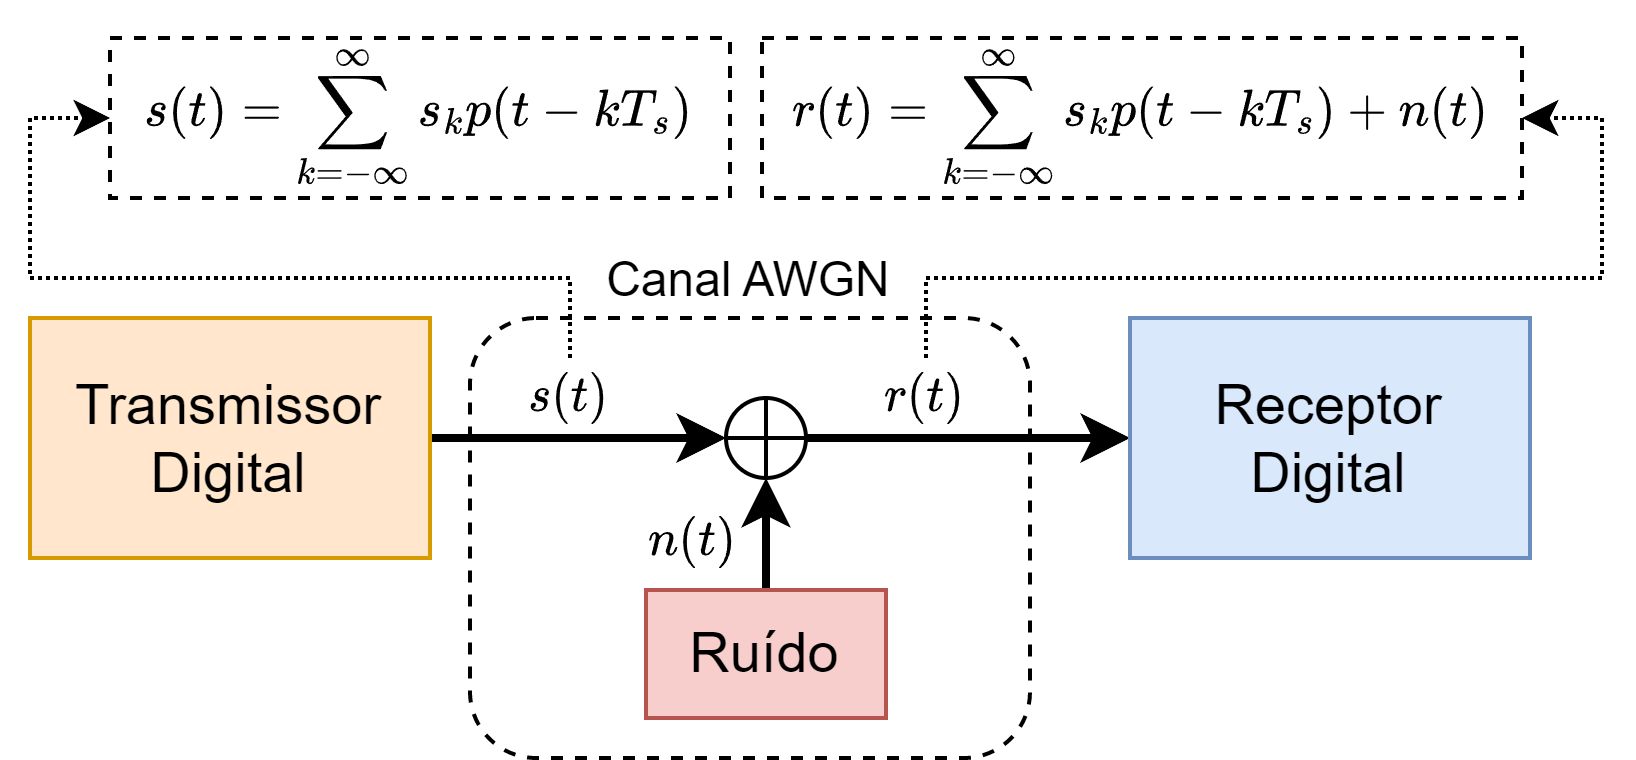
\includegraphics{figuras/Fig3.png}

em que \(r(t)\) representa o sinal ruidoso na entrada do receptor.

Uma das principais fontes de ruído em sistemas de comunicações é o ruído
térmico. O ruído Johnson-Nyquist (ruído térmico, ruído de Johnson ou
ruído de Nyquist) é o ruído eletrônico gerado pela agitação térmica dos
portadores de carga (geralmente os elétrons) dentro de um condutor
elétrico, que ocorre independentemente de haver ou não tensão aplicada
sobre o elemento. O ruído térmico está presente em todos os circuitos
elétricos e eletrônicos. A presença de ruído em circuitos eletônicos
reduz a sensibilidade de receptores na detecção de sinais de potência
reduzida. Alguns equipamentos eletrônicos que requerem alta
sensibilidade, como receptores de telescópios de rádio, precisam ser
resfriados à temperaturas criogênicas para reduzir o ruído térmico em
seus circuitos.

\begin{block}{Variável aleatória com distribuição gaussiana}
\phantomsection\label{variuxe1vel-aleatuxf3ria-com-distribuiuxe7uxe3o-gaussiana}
Seja \(X\) uma v.a. contínua com distribuição normal (gaussiana) de
média \(\mu\) e variância \(\sigma^2\),
i.e.~\(X \sim \mathcal{N}\mathrm{(\mu, \sigma^2)}\), a função densidade
de probablidade de \(X\) será dada por

\[
p_X\left(x\right)=\frac{1}{\sqrt{2 \pi \sigma^{2}}} e^{-\frac{(x-\mu)^{2}}{2 \sigma^{2}}}
\]

para \(-\infty <x < \infty\).

Exemplos:

Seja \(P(x_1 < X < x_2)\) a probabilidade de X assumir valores no
intervalo \([x_1, x_2]\), temos que

em que
\(\operatorname{erf}(x) =\frac{2}{\sqrt{\pi}} \int_0^x e^{-u^2} \mathrm{~d} u\).
\end{block}

\begin{block}{Processo estocástico gaussiano estacionário}
\phantomsection\label{processo-estocuxe1stico-gaussiano-estacionuxe1rio}
Um processo estocástico gaussiano estacionário \(X(t)\) é um processo
aleatório no qual a distribuição de probabilidade conjunta de qualquer
conjunto finito de variáveis aleatórias
\(\mathbf{X} = \left[X(t_1), X(t_2), \dots X(t_n) \right]^T\) possuirá
uma distribuição conjunta gaussiana, ou seja, uma função densidade de
probabilidade (fdp) dada por

\begin{equation} p_{\mathbf{X}}(\mathbf{x}) = \frac{1}{\sqrt{(2\pi)^n|\Sigma|}} e^{-\frac{1}{2} (\mathbf{x}-\mathbf{\mu})^T \Sigma^{-1} (\mathbf{x}-\mu)} \end{equation}\label{eq1}\]

onde \(\mathbf{x}\) é um vetor coluna de dimensão \(n\),
\(\mathbf{\mu}\) é um vetor coluna de médias de dimensão \(n\),
\(\Sigma\) é uma matriz de covariância \(n \times n\), \(|\Sigma|\) é o
determinante de \(\Sigma\) e \(^T\) representa a transposição. No caso
de processos gaussianos, se as variáveis aleatórias forem mutuamente
independentes,
\(\Sigma = \mathrm{diag}(\sigma_1^2, \sigma_2^2, \dots, \sigma_n^2)\)
será uma matriz diagonal e temos que (\(\ref{eq1}\)) pode ser
simplificada para

\begin{eqnarray} p_{\mathbf{X}}(\mathbf{x}) &=& p(x_1)p(x_2)\dots p(x_n) \\ &=&\prod_{k=1}^n \frac{1}{\sqrt{2\pi \sigma_k^2}} e^{-\frac{1}{2} \frac{(x_k-\mu_k)^2}{\sigma_k^2}} \end{eqnarray}\label{eq2}\]

A propriedade de estacionariedade em um processo estocástico implica que
suas estatísticas não variam ao longo do tempo. Em outras palavras, as
médias e variâncias das variáveis aleatórias do processo são constantes
temporalmente e as funções de autocorrelação e covariância dependem
apenas da diferença entre os instantes de tempo, não do tempo em si.
Essa propriedade é de grande importância na análise de processos
estocásticos, pois permite simplificar a modelagem e a análise de
sistemas complexos. Ao assumir que o processo é estacionário, podemos
reduzir a dimensão do problema e concentrar nossos esforços na
caracterização da estatística do processo em vez de sua dinâmica
temporal.
\end{block}

\begin{block}{Propriedades importantes:}
\phantomsection\label{propriedades-importantes}
\begin{enumerate}
\item
  Para processos gaussianos, o conhecimento da média e da
  autocorrelação, i.e., \(\mu_X(t)\) e \(R_X(t_1, t_2)\) provê uma
  descrição estatística completa do processo.
\item
  Se um processo gaussiano \(X(t)\) passa por um sistema linear e
  invariante no tempo (LIT), então a saída \(Y(t)\) do sistema também é
  um processo gaussiano.
\item
  Para processos gaussianos, estacionariedade no sentido amplo (WSS)
  implica em estacionariedade estrita.
\item
  Uma condição suficiente para a ergodicidade de um processo
  estacionário de média nula \(X(t)\) é que
\end{enumerate}

\[\int_{-\infty}^{\infty}\left|R_X(\tau)\right| d \tau<\infty\].
\end{block}
\end{frame}

\begin{frame}{Ruído aditivo gaussiano branco}
\phantomsection\label{ruuxeddo-aditivo-gaussiano-branco}
O ruído gaussiano branco \(N(t)\) é um processo estocástico estacionário
em que qualquer conjunto as amostras das realizações do processo são
independentes e identicamente distribuídas (i.i.d.) com uma distribuição
gaussiana de média zero e variância constante. O termo ``branco''
refere-se ao fato de que a densidade espectral de potência do processo
constante ao longo de todo o espectro de frequências, fazendo alusão à
luz branca, que é composta pela combinação de todas as componentes de
frequência (cores) do espectro visível.

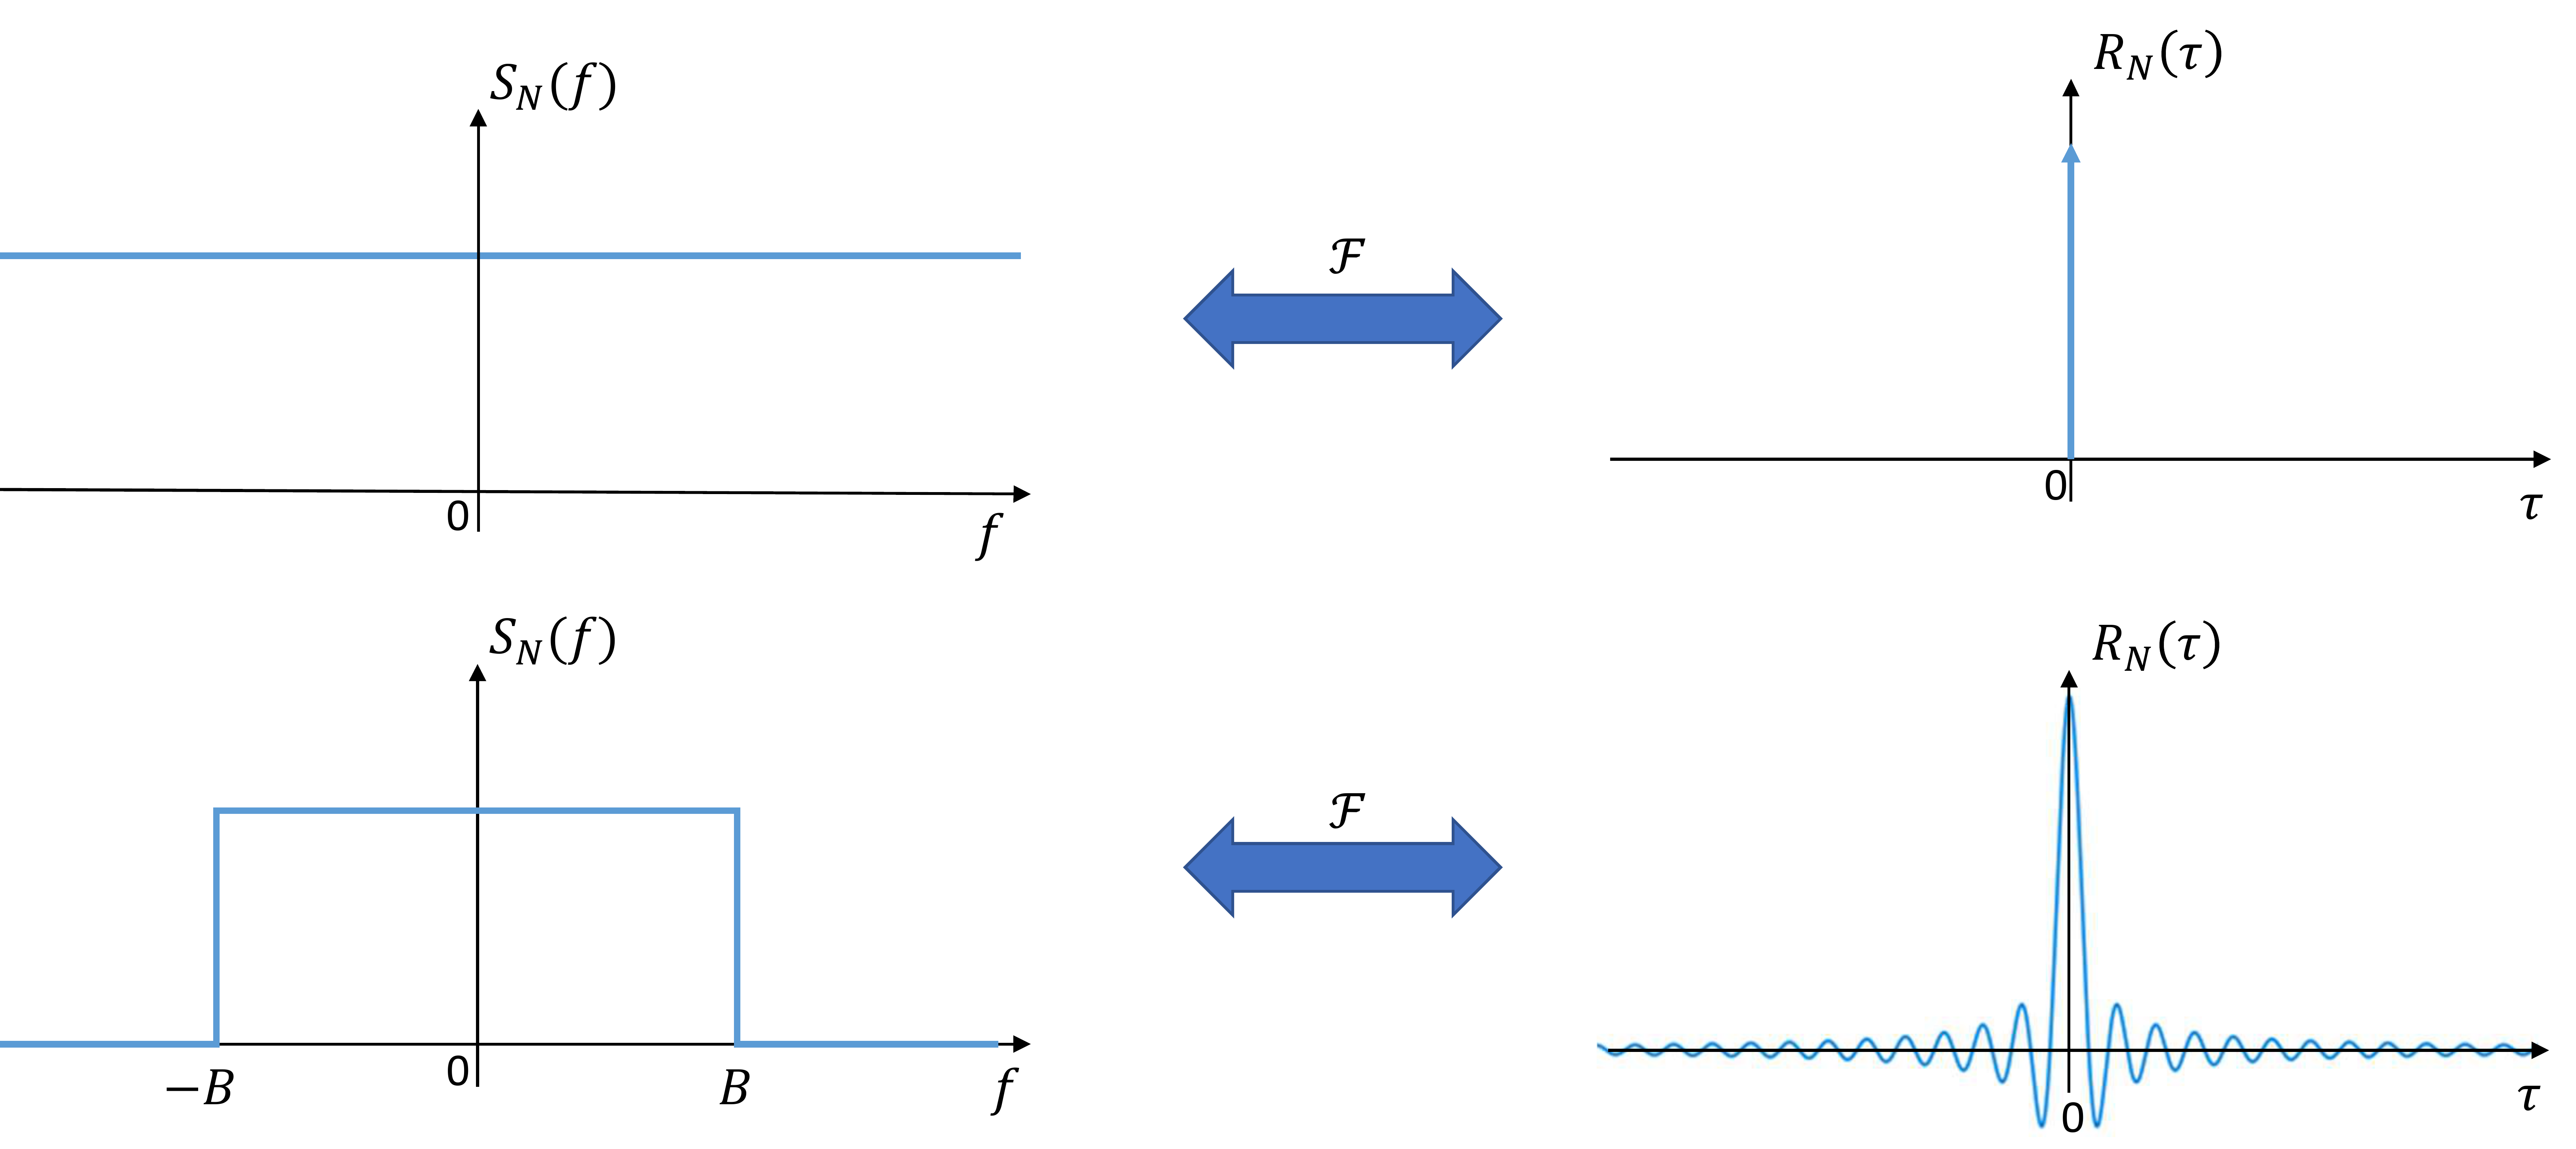
\includegraphics{figuras/Fig4.png}

\begin{block}{Filtrando o ruído gaussiano branco}
\phantomsection\label{filtrando-o-ruuxeddo-gaussiano-branco}
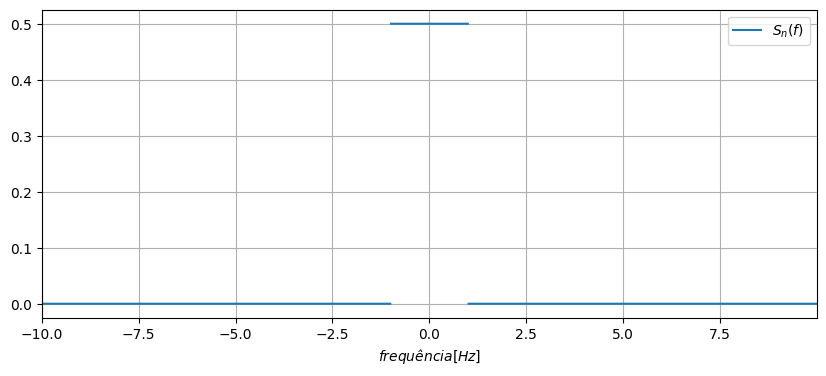
\includegraphics{figuras/nb1_out_0.png}

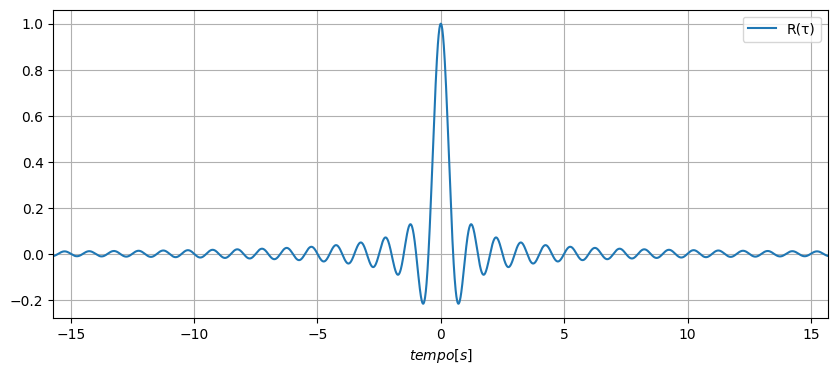
\includegraphics{figuras/nb1_out_1.png}
\end{block}

\begin{block}{Exemplo: ruído térmico}
\phantomsection\label{exemplo-ruuxeddo-tuxe9rmico}
A densidade de potência do ruído térmico é dada por

\[ S_n(f)=\frac{\hbar f}{2\left(e^{\frac{\hbar f}{k T}}-1\right)} \]

em que \(f\) é a frequência em \(Hz\),
\(\hbar=6.6 \times 10^{-34} \mathrm{~J}\mathrm{s}\) é a constante de
Planck, \(k=1.38 \times 10^{-23}  \mathrm{~J}\mathrm{K}\) é a constante
de Boltzmann e \(T\) é a temperatura em Kelvin.

Observações:

\begin{itemize}
\tightlist
\item
  O espectro acima assume valor máximo \(\frac{kT}{2}\) em \(f=0\) Hz;
\item
  \(\lim_{f\to \pm \infty} S_n(f) = 0\), porém a taxa de convergência é
  muito lenta. Ex.: a 300 K, \(S_n(f)=0.9S_n(0)\) para
  \(f=2\times 10^{12} Hz\)
\end{itemize}

Logo, para efeitos práticos:

\[ S_n(f)=\frac{kT}{2} \]

Considerando um intervalo de frequências \([-B/2, B/2]\), a potência de
ruído térmico presente nessa banda será dada por

\[
\begin{aligned}
& P_n=\int_{-B/2}^{B/2} \frac{k T}{2} d f \\
& P_n=\frac{k T}{2} \cdot 2 \frac{B}{2} =k T B/2
\end{aligned}
\]
\end{block}

\begin{block}{Gerando numericamente realizações de um processo
gaussiano}
\phantomsection\label{gerando-numericamente-realizauxe7uxf5es-de-um-processo-gaussiano}
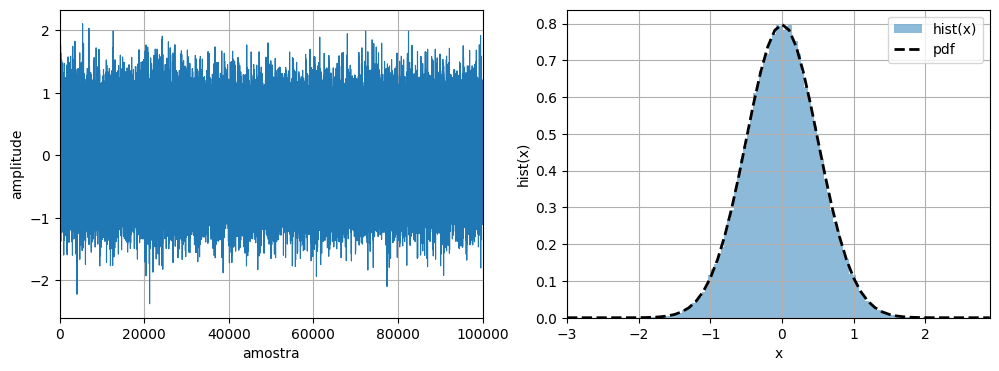
\includegraphics{figuras/nb1_out_2.png}

Veja que o sinal ilustrado acima é a realização de um processo
estocástico gaussiano estacionário. Cada amostra corresponde a uma
realização de uma variável aleatória (v.a) gaussiana de média nula
(\(\mu=0\)) e variância \(\sigma^2\). As variáveis aleatórias, por sua
vez, são independentes e idênticamente distribuídas (i.i.ds). Vamos
calcular a potência do sinal acima, considerando que para um processo
ergódico na correlação, podemos assumir:

\[P_x=E\left[X^2\right] = \mu^2 + \sigma^2\approx \frac{1}{N}\sum_{k=1}^{N} x^2[k]\]

Note que esta última expressão é a mesma expressão para cálculo da
potência média de um sinal determinístico. Logo, temos que:
\end{block}

\begin{block}{Efeito do ruído em sistemas de comunicação digital}
\phantomsection\label{efeito-do-ruuxeddo-em-sistemas-de-comunicauxe7uxe3o-digital}
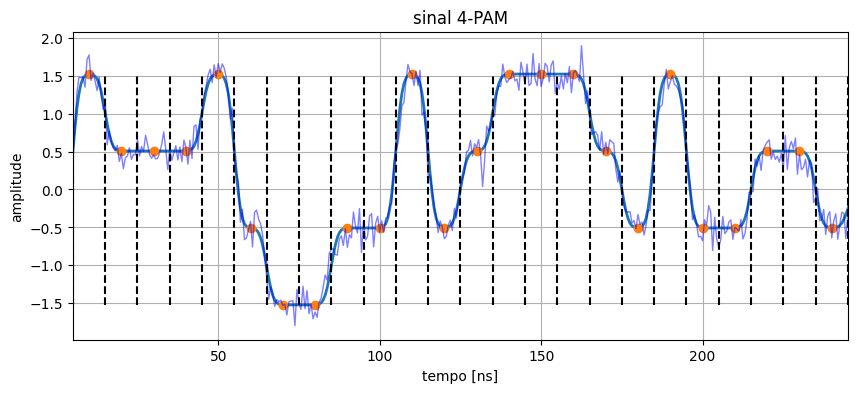
\includegraphics{figuras/nb1_out_3.png}

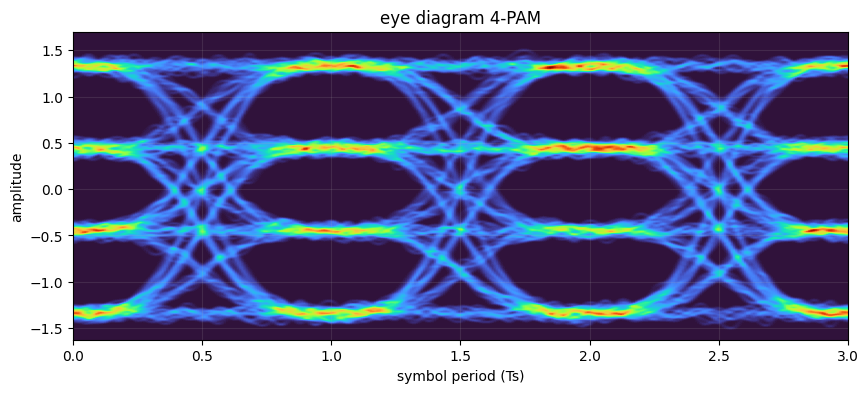
\includegraphics{figuras/nb1_out_4.png}
\end{block}
\end{frame}

\begin{frame}{Relação sinal-ruído}
\phantomsection\label{relauxe7uxe3o-sinal-ruuxeddo}
A relação sinal-ruído (ou razão sinal-ruído, \emph{signal-to-noise
ratio} - \(\mathrm{SNR}\)) é uma das grandezas mais importantes na
engenharia de sistemas de comunicações. A \(\mathrm{SNR}\) é um
indicador da presença de ruído no sistema, ou seja, a presença de
distorções aleatórias e indesejáveis que afetam os sinais que carregam
informação, dificultando ou impossibilitando o processo de comunicação.

A \(\mathrm{SNR}\) é definida como sendo a razão entre a potência de
sinal \(P_s\) e a potência do ruído \(P_n\) observadas num dado sistema:

\[\mathrm{SNR} = \frac{P_s}{P_n}\]

em que \(P_s = E\left[|s(t)|^2\right]\) e
\(P_n=E\left[|n(t)|^2\right]\), com \(E[.]\) denotando valor esperado.

Quando expressa em decibéis (dB), a \(\mathrm{SNR}\) é dada por

\[ \mathrm{SNR}_{dB} = 10\log_{10}P_s-10\log_{10}P_n.\]

Quanto maior a \(\mathrm{SNR}\) maior a diferença entre a potência do
sinal de interesse e a potência do ruído adicionado á mesma. Dessa
forma, quanto maior a \(\mathrm{SNR}\) melhor a qualidade do sinal.
\end{frame}

\begin{frame}{Referências}
\phantomsection\label{referuxeancias}
{[}1{]} J. G. Proakis, M. Salehi, Digital Communications, 4th Edition,
McGraw Hill, 2001.
\end{frame}

\end{document}
